\chapter{Design \& Specification} \label{Design}
  
% Provide abstract level of how I intend to compare them
% How do I make sure the implementation is like for like
% 

Here, I will provide an abstract level of how I compared the performance of each content generation algorithm and how I made sure each implementation could produce as similar/like-for-like results as possible (and where they \textit{couldn't} do so). I delve into more specifics and quantified data in Chapter \ref{Evaluation}.

\section{Performance}

With the L-System implementation, I had no problems running the game very quickly on my machine, and quickly got satisfactory results results.

While my Noise implementation was slower than my L-System implementation by a magnitude, 

With Poisson Disk Sampling, the higher the number of rejection samples (that is, the higher the maximum number of times a cell was sampled before it was either accepted or ultimately rejected), the longer it took to generate a complete level layout, and even, due to the nature of the tile map compared to the algorithm's \textit{usual} use (of scattering dots on a plane), it was not maximal (not all points had cells painted for them; some cells had their tiles overwritten as well). Using 8 rejection samples was usually enough to yield a satisfactory level layout while also keeping level creation times to a minimum.

Voronoï Cells took the longest to compute on average. Computations with the Euclidean distance measurement took longer than those measured with the Manhattan distance.

\section{Layouts}

Of the 4 implementations I made, the Noise and Poisson Disk Sampling implementation were by far the most similar, followed by the L-System implementation, and then the Voronoï Cells implementation, which was far and away the most unique.

While the noise implementations varied greatly depending on what settings were used, and the way the implementation was designed allowed for very many possibilities as to how the noise would turn out (and how it would affect the final level), the results that I found produced the most similar results to that of the Poisson Disk Sampling implementation had the following configurations:

\begin{itemize} \label{noisedefaults}
    \item Noise Type (``noise\_type"): Simplex Smooth
    \item Fractal Type (``fractal\_type"): Fractal None
    \item Cellular Distance Type/Function (``cellular\_distance\_type"): Distance Euclidean
    \item Noise Frequency (``noise\_frequency"): 0.894
    \item Tree Cap (``tree\_cap"): -0.048
    \item Building Cap (``building\_cap"): -0.252
    \item Building Overtakes Tree (``building\_overtakes\_tree"): 0.12
\end{itemize}

The default noise frequency in ``FastNoiseLite" is 0.01, which results in smoother and less disparate noise. As seen in Figure \ref{fig:simplexsmooth0.01}, the smoother noise and lower frequency results in a distinct kind of level layout in which  

\begin{figure}[H]
    \centering
    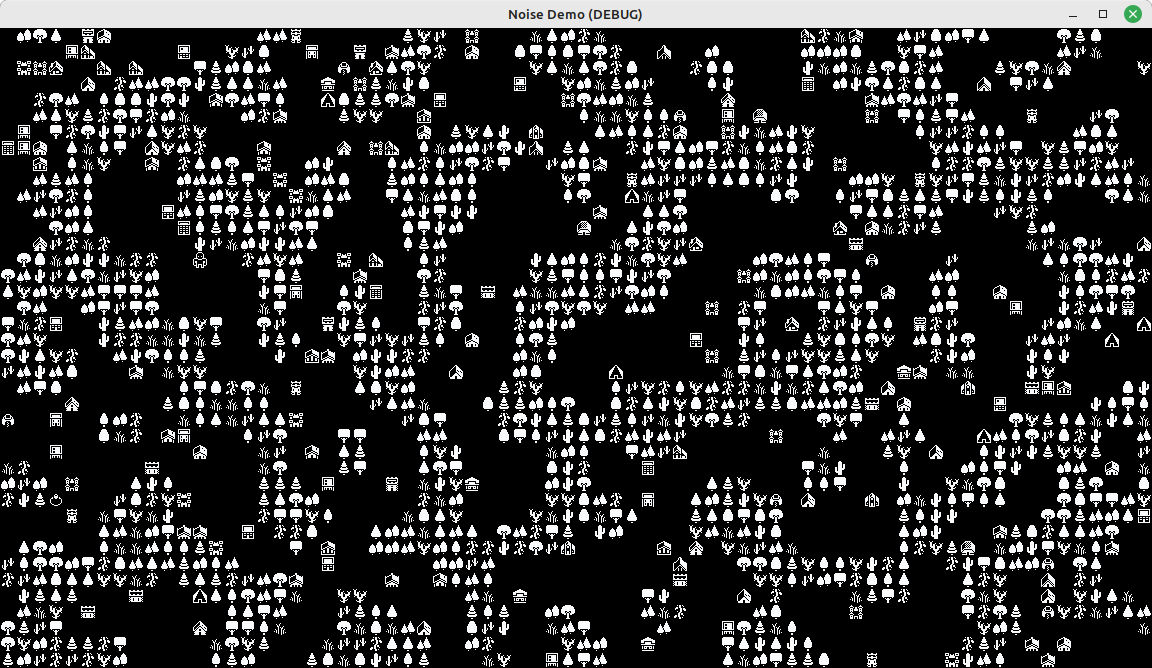
\includegraphics[width=\textwidth]{Images/simplex_smooth_0.01_frequency.png}
    \caption{A level of our scenario generated in the Simplex Noise implementation, setting the noise frequency to 0.01 (the default value for noise frequency in ``FastNoiseLite") and using the rest of the defaults \hyperref[noisedefaults]{shown here}. The level took a total of 104 milliseconds to be made.}
    \label{fig:simplexsmooth0.01}
\end{figure}